\documentclass[aspectratio=169]{beamer}
\usepackage{enumitem}
\usepackage{bm}
\usepackage{amsfonts}
\usepackage{float}
\usepackage[config, labelfont={bf}]{caption,subfig} % nice sub figures
\renewcommand{\baselinestretch}{1.0} 	 % line Spacing
\setbeamertemplate{footline}[frame number]

\newcommand{\nudge}{\hspace{0.01in}}

\title{Efficient Simulation Of A Simple Evolutionary System}
\author{Mahendra Duwal Shrestha}
\institute{The University Of Tenessee}
\date{\today}


\begin{document}

  \begin{frame}
    \titlepage
  \end{frame}

  \begin{frame}
    \frametitle{Outline}
    \begin{itemize}
      \item{Background}
      \item{Question 1: Convergence of finite population}
      \item{Question 2: Oscillation in finite population}
      \item{Question 3: Oscillation in finite population under mutation-violation}
      \item{Question 4: Oscillation in finite population under crossover-violation}
      \item{Conclusion}
    \end{itemize}
  \end{frame}

  \begin{frame}
    \frametitle{Terms}
    \begin{itemize}
      \item{Population $P$: a collection of length $\ell$ binary strings}
      \item{Population vector $\bm{p}$: $\bm{p}_j$ is the proportion of string $j$ in the population}
      \item{If $P \,=\, {00, 01, 01, 10, 11, 11}$, then $\bm{p}_3 \,=\, 2/6 \,=\, 1/3$}
      \item{$\mathcal{R}$ denotes a set binary strings of length $\ell$, $|\mathcal{R}| = Z = 2^\ell$ }
      \begin{itemize}
	\item{Addition and multiplication of elements in $\mathcal{R}$ are bitwise operations modulo 2}
	\item{$x \,=\, 1101,\, y \,=\, 1010 $}
	\item{$x + y \,=\, 1101 + 1010 \,=\, 0111$}
	\item{$xy \,=\, 1101 \cdot 1010 \,=\, 1000$}
	\item{$\bar{x} \,=\, 0010$}
      \end{itemize}
    \end{itemize}
  \end{frame}
  
  \begin{frame}
    \frametitle{Crossover \& Mutation}
    \begin{itemize}
      \item{Crossover : Choose parents $u$ and $v$, exchange bits using crossover mask $m$: }
      \item{$u^\prime \,=\, um + v\bar{m} , v^\prime \,=\, u\bar{m} + vm$}      
      \item{$u = \bm{1100}, v = 1101, m = 1100$}
      \item{$\{\bm{1100}, 1101\} \to \{\bm{11}00 + 0001,\, 00\bm{00} + 1100\} \to \{\bm{11}01, 11\bm{00}\}$}
      \item
      \item{Mutation: Flip bits using mutation mask:}
      \item{$x \to x + m$}
      \item{$x = 1100, m = 0001$}
      \item{$1100 \to 1100 + 0001 \to 1101$}
    \end{itemize}
  \end{frame}
  
  \begin{frame}
    \frametitle{Finite Population GA}
    \begin{columns}
          \column{0.30\linewidth}
             \centering
             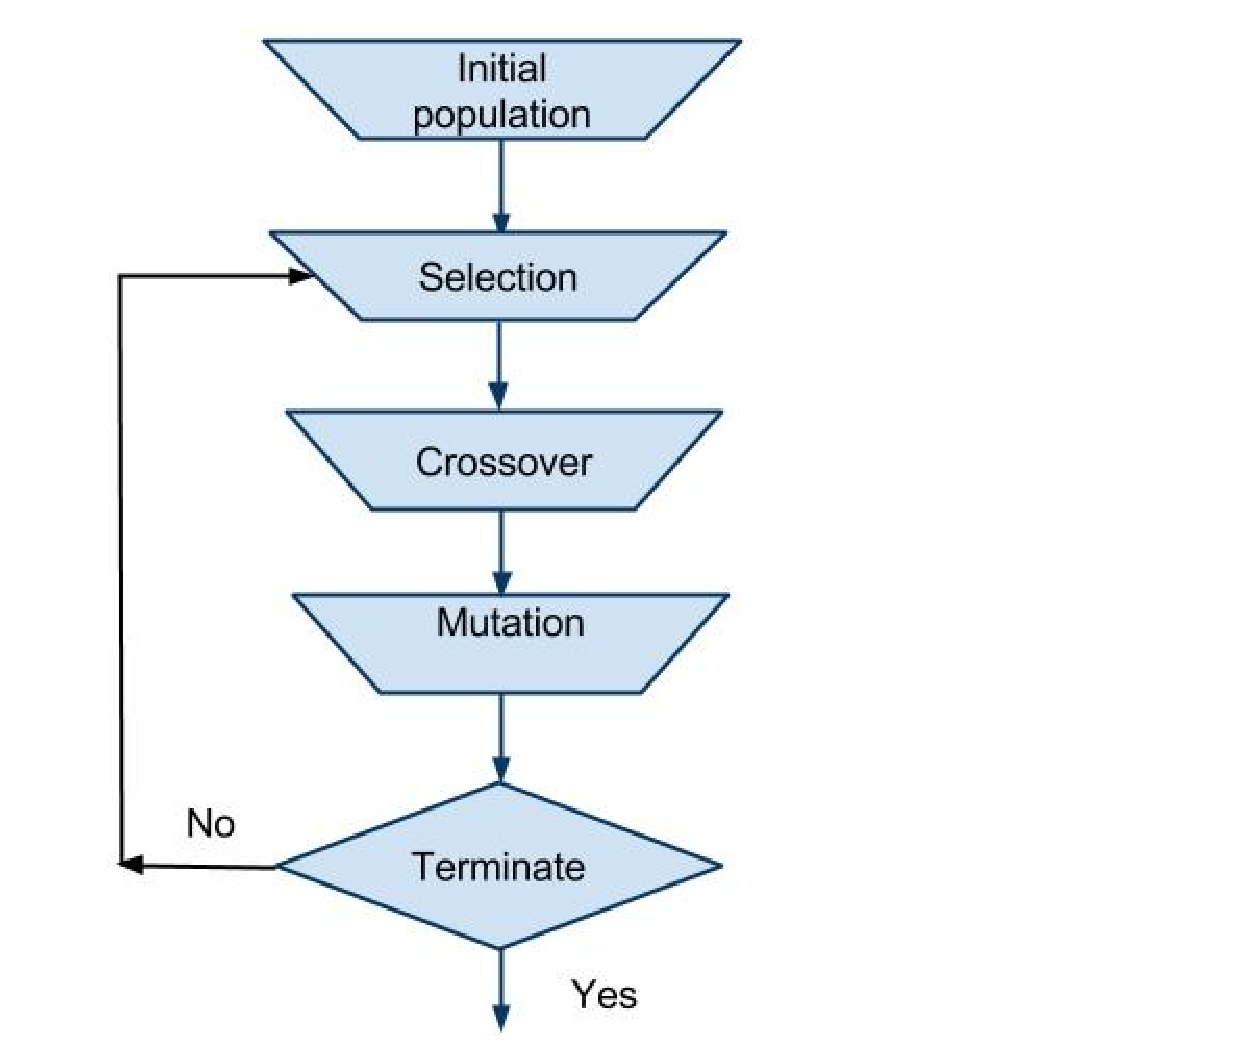
\includegraphics[height=6cm, width=5cm]{figures/eps/GA.eps}
           \column{0.67\linewidth}
	    \begin{itemize}
              \item{Randomly select parents $u$ and $v$ }
              \item{Crossover $u$ and $v$ to produce $u^\prime$ and $v^\prime$ }
              \item{Keep one of $u^\prime$, $v^\prime$ , and mutate to produce gamete $g$}
              \item{Repeat above to form next generation}              
	    \end{itemize}
         \end{columns} 
  \end{frame}
  
  \begin{frame}
    \frametitle{Random Heuristic Search}
    \begin{itemize}
      \item{$\tau$ is a stochastic transition rule that maps 
      $\bm{p}$ to $\bm{p^\prime} \in \Omega_N = \{\langle \frac{X_1}{N},\cdots,\frac{X_Z}{N} \rangle |X_i \in \mathcal{I} \geq 0, \sum X_i = N\}$}
      \item{For a finite population, sequence $\bm{p}, \tau(\bm{p}), \tau^2(\bm{p}), \cdots $ forms Markov chain}
      \item{$\tau(\bm{p})$ cannot be predicted with certainty }      
      \item{$\bm{\chi}_i \,=\,$ probability of using crossover mask $i$ }
      \item{$\bm{\mu}_i \,=\,$ probability of using mutation mask $i$ }
    \end{itemize}
  \end{frame}
  
  \begin{frame}
    \frametitle{Infinite Population Model}
    \begin{itemize}
      \item{Population is modeled as a vector $\bm{p} \in \Omega = \{\langle \bm{p}_1, \cdots \bm{p}_Z \rangle | \bm{p}_i \geq 0, \sum \bm{p}_i = 1 \}$}
      \item{$\mathcal{G}$ maps $\bm{p}$ to the next generation}
      \item{$\mathcal{G}(\bm{p})_j$ =  probability that string $j$ occurs in the next generation}
      \item{The infinite population model is the sequence }
      \item{$\bm{p} \to \mathcal{G}(\bm{p}) \to  {\mathcal{G}}(\mathcal{G}(\bm{p})) \to \cdots $}
      \item{The variance in the next generation  is
	\[\mathcal{E}(\| \tau (\bm{p}) - \mathcal{G}(\bm{p}) \|^2) = \frac{1 - \|\mathcal{G}(\bm{p})\|^2}{N}\]
      }
    \end{itemize}  
  \end{frame}  
  
  
  \begin{frame}
    \frametitle{Question 1: Distance Between Finite and Infinite Population}
    \begin{itemize}
      \item{Chebyshev's inequality $\to$ \[ \| \tau (\bm{p}) - \mathcal{G}(\bm{p}) \| \,\leq\, \frac{k}{\sqrt{N}} \] }
      \item{Jensen's inequality  
      $\to$ \[ \mathcal{E}(\| \tau (\bm{p}) - \mathcal{G}(\bm{p}) \| \,\leq\, \frac{\sqrt{1 - \|\mathcal{G}(\bm{p})\|^2}}{\sqrt{N}}\]}
      \item{Geometric point of view $\to$ \[ \sup \; \inf \|\bm{\xi} - \bm{p}\| \;=\; O(1/\sqrt{N}) \] 
	$\bm{\xi} \in \Omega,\, \bm{p} \in \Omega_N$
      }      
    \end{itemize}
%     \newline
%     \newline
      \mbox{}\\[0.25 in]
    Does the distance decrease in practice like $1/\sqrt{N}$ ?
  \end{frame}
  
  \begin{frame}
    \frametitle{Diploid Population Model}
    \begin{itemize}
      \item{Diploid genome: $\quad \alpha \,= \langle \alpha_0, \alpha_1 \rangle$}
      \item{$\bm{q} \, \to \,$ current population} 
      \item{$\bm{q}_\alpha \, \to \,$ prevalence of diploid $\alpha$}
      \item{$t_\alpha(g) \, \to\,$ probability that gamete $g$ is produced from parent $\alpha$ }
      \item{\[\bm{q}_\gamma^{\prime} \; = \;
      \sum_{\alpha} \, \bm{q}_\alpha \, t_\alpha(\gamma_0) 
      \sum_{\beta} \,\bm{q}_\beta \, t_\beta(\gamma_1)\]}
    \end{itemize}
  \end{frame}
  
  \begin{frame}
    \frametitle{Diploid Model Reduction to Haploid Model}
    \begin{itemize}
      \item{Diploid distribution in terms of haploids
      \[\bm{q}_{\langle \gamma_0, \gamma_1 \rangle}\; = \;
      \bm{p}_{\gamma_0} \, \bm{p}_{\gamma_1}\]}
      \item{Haploid distribution in terms of diploids
      \[ \bm{p}_g \, = \, \frac{1}{2} \sum_{\alpha_0, \, \alpha_1} \, \bm{q}_{\langle \alpha_0, \alpha_1 \rangle}
	    ([g = \alpha_0] + [g = \alpha_1]) \]}
      \item{Evolution equation in terms of haploid distributions $\bm{p}$,
      \[\bm{p}_{\gamma_0}^{\prime} \,=\, \sum_{\alpha_0, \, \alpha_1} \, \bm{p}_{\alpha_0} \, \bm{p}_{\alpha_1} \,
	  t_{\langle \alpha_0, \,\alpha_1 \rangle}(\gamma_0) \]}
      \item{Matrix form:
      \[ \bm{p}_g^\prime \; = \; \bm{p}^T M_g \, \bm{p} \] where \[ \Big(M_g \Big)_{u,v} \; = \; t_{\langle u, v \rangle}(g) \]}
    \end{itemize}
  \end{frame}
  
  \begin{frame}
    \frametitle{Specialization to Vose's Haploid Model}
    \begin{itemize}
      \item{Mutation distribution: \[\bm{\mu}_i = (\mu)^{{\bf 1}^Ti} (1-\mu)^{\ell- {\bf 1}^Ti} \]}
      \item{Crossover distribution: \[
	\bm{\chi}_i =\begin{cases}
	  \chi c_i & \text{if $i>0$}\\
	  1 - \chi + \chi  c_0 & \text{if $i = 0$}
	\end{cases}
      \]}
      \item{For uniform crossover, $c_i = 2^{-\ell}$}
      \item{\[ t_{\langle u,v \rangle}(g) \; = \;\,
      \sum_{i \nudge \in \nudge \mathcal{R}} \, \sum_{j \nudge \in \nudge \mathcal{R}} \,
      \sum_{k \nudge \in \nudge \mathcal{R}}
      \bm{\mu}_i \nudge \bm{\mu}_j \, \frac{\bm{\chi}_k + \bm{\chi}_{\overline{k}}}{2} \,
      [\nudge k (u + i) + \overline{k}(v + j) \, = \, g\nudge] \] where $u,v \in \mathcal{R}$}
      
    \end{itemize}
  \end{frame}
  
  \begin{frame}
    \frametitle{Walsh Basis}
    \begin{itemize}
	\item{$W_{n,t} = Z^{-1/2} (-1)^{n^T t}$ where $Z = 2^\ell$}
	\item{$\widehat{A} = WAW$}
	\item{$\widehat{w} = Ww$}
	\item{Mixing matrix in Walsh basis 
	\[
	  \widehat{M}_{u,v} \; = \; 2^{\,\ell-1} \,[\nudge u \nudge v = {\bf
	  0}\nudge]\, \widehat{\bm{\mu}}_u \nudge \widehat{\bm{\mu}}_v \!  \sum_{k
	\nudge \in \nudge \overline{u+v} \nudge \mathcal{R}} \bm{\chi}_{k + u} +
	\bm{\chi}_{k + v}
	\]
	}
	\item{Evolution eqn in Walsh basis 
	\[
	  \widehat{\bm{p}}_g^{\,\,\prime} \; = \; 2^{\,\ell/2} \sum_{i \nudge \in \nudge g \mathcal{R}}
	  \widehat{\bm{p}}_i \, \nudge \widehat{\bm{p}}_{i+g} \,\widehat{M}_{i,i+g}
	\]
	 where $g \mathcal{R} = \{g \nudge i \, | \, i \in \mathcal{R} \}$
	}
    \end{itemize}
  \end{frame}
  
  \begin{frame}
    \frametitle{Computational Advantages}
    \begin{itemize}
      \item{Specialization simplifies computation, which otherwise for diploid case would have been impractical} 
      \item{Only one mixing matrix as opposed to $2^\ell$ is needed to compute next generation}
      \item{For $\ell = 14$, using $2^{14}$ mixing matrices with each having $2^{14} \cdot 2^{14}$ 
      entries would require 32 TB of memory, whereas one mixing matrix requires only 2 GB}
    \end{itemize}
  \end{frame}
  
  \begin{frame}
    \frametitle{Distance Computation}
    \begin{itemize}      
      \item{Naive computation 
      \[
	\|{\bm f} - {\bm q} \hspace{0.005in} \|^2 \; = \;
	  {\sum_{\alpha}} ({\bm f}_\alpha-{\bm q}_\alpha)^2 
	   \xrightarrow{\hspace*{1cm}} 2^\ell \cdot 2^\ell \, terms 
	\]}
      \item{Our implementation
	\begin{equation*}
	  \|{\bm f} - {\bm q} \hspace{0.005in} \|^2 \; = \; {\sum_{g}}^2 ({\bm p}_{g})^2 \, +
	  \sum_{\alpha \in {S_{\bm f}}} {\bm f}_\alpha ({\bm f}_\alpha- 2 {\bm q}_\alpha) \to 2^\ell + |S_{\bm f}| \, terms 
	\end{equation*}
      }
      \item{\[
	      S_{\bm f} \; = \; \{ \alpha \, | \, {\bm f}_\alpha > 0 \}
	      \]
      }
    \end{itemize}
  \end{frame}
  
  \begin{frame}
    \frametitle{Convergence}  
      \[\chi \,=\, 0.1, \; \mu \,=\, 0.001\]
	\begin{figure}[!hb]
	  \begin{center}
	    \subfloat[$\ell = 4$]{
	    \resizebox*{3cm}{!}{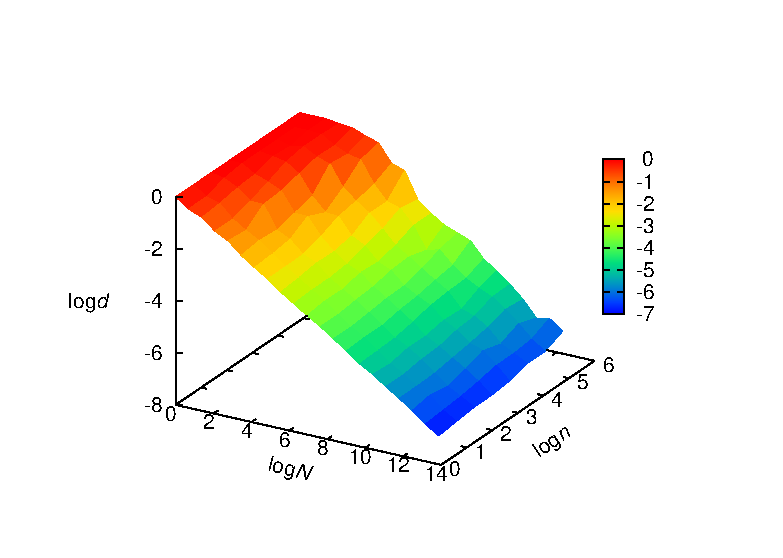
\includegraphics{figures/eps/surf/b4.eps}}}\hspace{5pt}
	    \subfloat[$\ell = 6$]{
	    \resizebox*{3cm}{!}{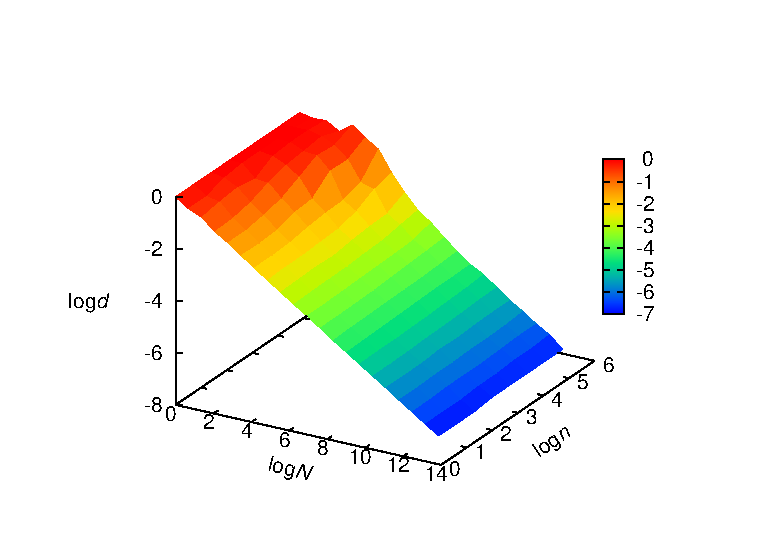
\includegraphics{figures/eps/surf/b6.eps}}}\hspace{5pt}
	    \subfloat[$\ell = 8$]{
	    \resizebox*{3cm}{!}{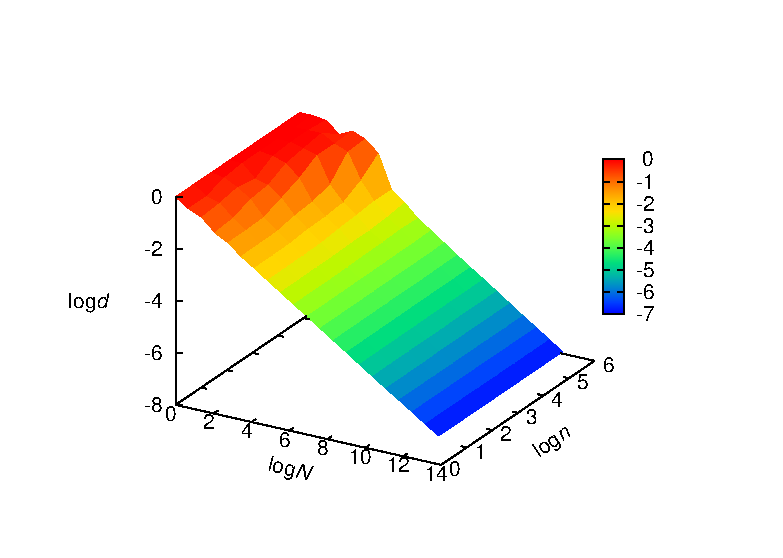
\includegraphics{figures/eps/surf/b8.eps}}}
	  \end{center}
	  \begin{center}
	  \subfloat[$\ell = 10$]{
	    \resizebox*{3cm}{!}{\includegraphics{figures/eps/surf/b10.eps}}}\hspace{5pt}
	    \subfloat[$\ell = 12$]{
	    \resizebox*{3cm}{!}{\includegraphics{figures/eps/surf/b12.eps}}}\hspace{5pt}
	    \subfloat[$\ell = 14$]{
	    \resizebox*{3cm}{!}{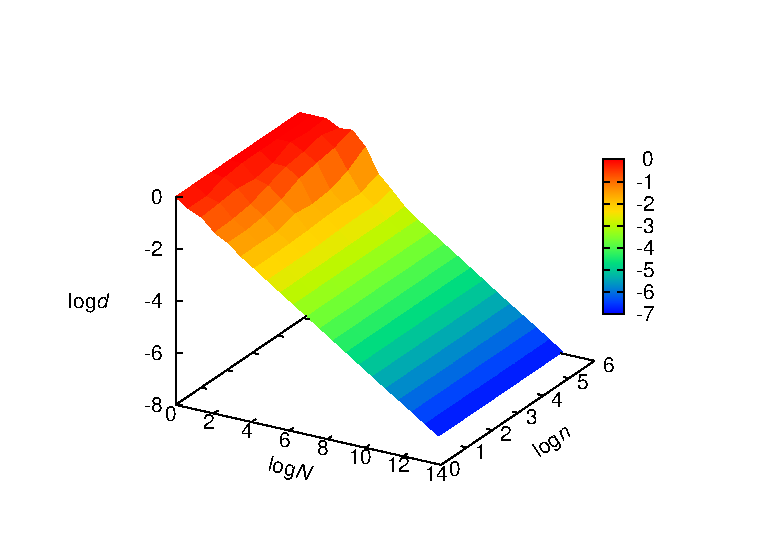
\includegraphics{figures/eps/surf/b14.eps}}}
	    \caption[]{Convergence of finite population behaviour}   
	  \end{center}
	\end{figure}      
    
  \end{frame}
  
  \begin{frame}
    \frametitle{Regression}
    \[\log d = m \log N + b\]
    \mbox{}\\[-0.5in]
    \begin{figure}[!ht]
      \begin{center}
	\subfloat[Slope $m$]{
	\resizebox*{4cm}{!}{\includegraphics{figures/eps/slope/m.eps}}}\hspace{5pt}
	\subfloat[Intercept $b$]{
	\resizebox*{4cm}{!}{\includegraphics{figures/eps/slope/b.eps}}}
	\caption[]{Regression parameter for generation $n \in \{1, 2, 4, 8, 16, 32, 64, 128\}$ }	
      \end{center}
    \end{figure}
    $d \approx N^m e^b$
    \newline
    From figure (a) above, $m \approx -0.5$ 
    \newline
    $d \approx k / √N$
  \end{frame}  
  
  \begin{frame}
    \frametitle{Does the distance between finite and infinite population decrease like $1/\sqrt{N}$}
    \begin{itemize}
      \item Yes
    \end{itemize}
  \end{frame}
  
  \begin{frame}
    \frametitle{Question 2}
    \begin{itemize}
      \item{Oscillation in Finite Populations}      
    \end{itemize}
  \end{frame}
  
  \begin{frame}
    \frametitle{Limits}
    \begin{itemize}
      \item{The sequence $\bm{p}, \, \mathcal{G}(\bm{p}), \, {\mathcal{G}}^2(\bm{p}), \, \cdots$ may converge to a fixed point }  
      \item{$\mathcal{G}(\omega) = \lim_{n\to\infty} \mathcal{G}^n(\bm{p}) = \omega$}
      \item{But under some circumstances, the sequence converges to a periodic orbit that oscillates between two fixed points, $\bm{p}^\ast$ and $\bm{q}^\ast$}
    \end{itemize}
  \end{frame}
  
  \begin{frame}
    \frametitle{Periodic Orbit: Necessary and Sufficient Conditions}
    \begin{itemize}
      \item{For some $g \,\in\, \mathcal{R} , g \,\neq\, 0$}    
      \item{
      \begin{eqnarray*}
      -1 &=& \sum \limits_{j} (-1)^{g^T j} \bm{\mu}_j \\
      1 &=& \sum \limits_{k \in \bar{g}\mathcal{R}} \bm{\chi}_{k+g} + \bm{\chi}_k 
      \end{eqnarray*}
      }
      \item{Infinite populations converge to a periodic orbit }
      \item{Do finite populations also exhibit oscillation from random initial populations?}
    \end{itemize}
  \end{frame}  
  
  \begin{frame}
    \frametitle{Previous Works on Oscillation}
    \begin{itemize}
      \item{Akin (1982) proved existence of cycling for continuous-time 2-bit diploid model}  
      \item{Hasting (1981) studied cycling in populations with infinite 2-bit diploid population model}
      \item{Wright and Bidwell (1997) provided examples of cycling in an infinite haploid model 
      with crossover and mutation for 3 bit and 4 bit populations }
      \item{Wright and Agapie (2001) described cycling in infinite population for up to 4 bits, 
      and also presented data for cycling in finite population}
    \end{itemize}
  \end{frame}
  
  \begin{frame}
    \frametitle{Difference From Previous Works}
    \begin{itemize}
      \item{Akin considered continuous time model and we consider discrete time model}
      \item{Hastings' study was limited to two bits length, and includes only crossover but not mutation}
      \item{Examples provided by Wright and Bidwell were for specific set parameter values for crossover, mutation and fitness }
      \item{Wright and Agapie used dynamic mutation that depends upon where population is in the population space}
      \item{Another difference between Wright and Agapie's work and ours is fitness}
      \item{We study cyclic behavior for:}      
      \begin{itemize}
	\item{fixed fitness function and random: initial population, mutation and crossover distribution}
	\item{higher bit length (up to 14)}
	\item{both haploid and diploid populations, and for both finite and infinite populations}
      \end{itemize}
      \item{We also visualize oscillation}
    \end{itemize}
  \end{frame}
  
  \begin{frame}
    \frametitle{Simulation}
    \begin{itemize}
      \item{Simulations were run for both haploid and diploid populations}
      \item{Random initial population}     
      \item{$\ell \;\in\; {8, 10, 12, 14}$}
      \item{$N \;=\; {4096, 40960, 81920}$}
      \item{To visualize oscillation, distances of population to fixed points $\bm{p}^\ast$ and $\bm{q}^\ast$ are plotted}
    \end{itemize}
  \end{frame}
  
  \begin{frame}
    \frametitle{Oscillation}
    \begin{figure}[!h]
      \begin{center}
	\subfloat{
	\resizebox{4cm}{2cm}{\includegraphics{figures/eps/osc/b8/n004096_osc_fin_hap.eps}}} \hspace{-2.3em}% 
	\subfloat{
	\resizebox{4cm}{2cm}{\includegraphics{figures/eps/osc/b8/n040960_osc_fin_hap.eps}}} \hspace{-2.3em}% 
	\subfloat{
	\resizebox{4cm}{2cm}{\includegraphics{figures/eps/osc/b8/n081920_osc_fin_hap.eps}}} \hspace{-2.3em}% 
	\subfloat{
	\resizebox{4cm}{2cm}{\includegraphics{figures/eps/osc/b8/osc_inf_hap.eps}}} \vspace{-1em} \hspace{-2.3em}%
	
      \end{center}
      \begin{center}
	\subfloat{
	\resizebox{4cm}{2cm}{\includegraphics{figures/eps/osc/b8/n004096_osc_fin_dip.eps}}}  \hspace{-2.3em}% 
	\subfloat{
	\resizebox{4cm}{2cm}{\includegraphics{figures/eps/osc/b8/n040960_osc_fin_dip.eps}}} \hspace{-2.3em}% 
	\subfloat{
	\resizebox{4cm}{2cm}{\includegraphics{figures/eps/osc/b8/n081920_osc_fin_dip.eps}}}  \hspace{-2.3em}% 
	\subfloat{
	\resizebox{4cm}{2cm}{\includegraphics{figures/eps/osc/b8/osc_inf_dip.eps}}} \vspace{-0.5em} \hspace{-2.3em}% 
	
      \caption[]{Infinite and finite population behavior for genome length $\ell = 8$}     
      \end{center}
    \end{figure}
  \end{frame}
  
  \begin{frame}
    \frametitle{Oscillation}
    \begin{figure}[!h]
      \begin{center}
	\subfloat{
	\resizebox{4cm}{2cm}{\includegraphics{figures/eps/osc/b12/n004096_osc_fin_hap.eps}}} \hspace{-2.3em}% 
	\subfloat{
	\resizebox{4cm}{2cm}{\includegraphics{figures/eps/osc/b12/n040960_osc_fin_hap.eps}}} \hspace{-2.3em}% 
	\subfloat{
	\resizebox{4cm}{2cm}{\includegraphics{figures/eps/osc/b12/n081920_osc_fin_hap.eps}}} \hspace{-2.3em}% 
	\subfloat{
	\resizebox{4cm}{2cm}{\includegraphics{figures/eps/osc/b12/osc_inf_hap.eps}}} \vspace{-1em} \hspace{-2.3em}%
	
      \end{center}
      \begin{center}
	\subfloat{
	\resizebox{4cm}{2cm}{\includegraphics{figures/eps/osc/b12/n004096_osc_fin_dip.eps}}}  \hspace{-2.3em}% 
	\subfloat{
	\resizebox{4cm}{2cm}{\includegraphics{figures/eps/osc/b12/n040960_osc_fin_dip.eps}}} \hspace{-2.3em}% 
	\subfloat{
	\resizebox{4cm}{2cm}{\includegraphics{figures/eps/osc/b12/n081920_osc_fin_dip.eps}}}  \hspace{-2.3em}% 
	\subfloat{
	\resizebox{4cm}{2cm}{\includegraphics{figures/eps/osc/b12/osc_inf_dip.eps}}} \vspace{-0.5em} \hspace{-2.3em}% 
	
      \caption[]{Infinite and finite population behavior for genome length $\ell = 12$}     
      \end{center}
    \end{figure}
  \end{frame}  
  
  \begin{frame}
    \frametitle{Oscillation: Conclusion}
    \begin{itemize}
      \item{Finite populations exhibit approximate oscillations}    
      \item{As population size increases, randomness decreases}      
    \end{itemize}
  \end{frame}
  
  \begin{frame}
    \frametitle{Question 3}
    \begin{itemize}
      \item{Oscillation Under Mutation-Violation}
      \item{
	\[
	  -1 \neq \sum \limits_{j} (-1)^{g^T j} \bm{\mu}_j      
	\]
      }
    \end{itemize}
  \end{frame}
  
  \begin{frame}
    \frametitle{Violation in Mutation}
    \begin{itemize}
      \item{Violation $\epsilon$ is introduced in $\bm{\mu}$}      
      \item{$\bm{\mu}_0 \,=\, \epsilon$}
      \item{$\bm{\mu}_i \,:=\, (1 \,-\, \epsilon)\bm{\mu}_i$}
      \item{This modification makes the Markov chain regular}
      \item{No periodic orbits for finite population}
      \item{No periodic orbits for infinite population}
      \item{Can finite population exhibit approximate oscillations?}
    \end{itemize}
  \end{frame}
  
  
  \begin{frame}
    \frametitle{Simulation}
    \begin{itemize}
      \item{$\epsilon$ = {0.01, 0.1, 0.5}}      
      \item{$\ell \,=\, \{8, 10, 12, 14\}$}
      \item{$N \,=\, \{4096, 40960, 81920\}$}
      \item{Distances of population to limits $p^\ast$ and  $q^\ast$ without violation are plotted }
    \end{itemize}
  \end{frame}
  
  \begin{frame}
    \frametitle{Results: Violation in Mutation}
    \mbox{}\\[-0.4in]
    \begin{figure}[!h]
      \begin{center}
	\subfloat{
	\resizebox{4cm}{2.5cm}{\includegraphics{figures/eps/vio/mu/b8/e0.01/n00004096_fin_hap_wovio.eps}}} \hspace{-2.3em}%
	\subfloat{
	\resizebox{4cm}{2.5cm}{\includegraphics{figures/eps/vio/mu/b8/e0.01/n00040960_fin_hap_wovio.eps}}} \hspace{-2.3em}%
	\subfloat{
	\resizebox{4cm}{2.5cm}{\includegraphics{figures/eps/vio/mu/b8/e0.01/n00081920_fin_hap_wovio.eps}}} \hspace{-2.3em}%
	\subfloat{
	\resizebox{4cm}{2.5cm}{\includegraphics{figures/eps/vio/mu/b8/e0.01/inf_hap_wovio.eps}}} \vspace{-0.8em} %
      \end{center}
      \begin{center}
	\subfloat{
	\resizebox{4cm}{2.5cm}{\includegraphics{figures/eps/vio/mu/b8/e0.1/n00004096_fin_hap_wovio.eps}}} \hspace{-2.3em}%
	\subfloat{
	\resizebox{4cm}{2.5cm}{\includegraphics{figures/eps/vio/mu/b8/e0.1/n00040960_fin_hap_wovio.eps}}} \hspace{-2.3em}%
	\subfloat{
	\resizebox{4cm}{2.5cm}{\includegraphics{figures/eps/vio/mu/b8/e0.1/n00081920_fin_hap_wovio.eps}}} \hspace{-2.3em}%
	\subfloat{
	\resizebox{4cm}{2.5cm}{\includegraphics{figures/eps/vio/mu/b8/e0.1/inf_hap_wovio.eps}}}\vspace{-0.8em} %
      \end{center}
      \begin{center}
	\subfloat{
	\resizebox{4cm}{2.5cm}{\includegraphics{figures/eps/vio/mu/b8/e0.5/n00004096_fin_hap_wovio.eps}}} \hspace{-2.3em}%
	\subfloat{
	\resizebox{4cm}{2.5cm}{\includegraphics{figures/eps/vio/mu/b8/e0.5/n00040960_fin_hap_wovio.eps}}} \hspace{-2.3em}%
	\subfloat{
	\resizebox{4cm}{2.5cm}{\includegraphics{figures/eps/vio/mu/b8/e0.5/n00081920_fin_hap_wovio.eps}}} \hspace{-2.3em}%
	\subfloat{
	\resizebox{4cm}{2.5cm}{\includegraphics{figures/eps/vio/mu/b8/e0.5/inf_hap_wovio.eps}}}\vspace{-0.8em} %      
      
      \caption[]{Infinite and finite haploid population behavior for $\bm{\mu}$ violation and $\ell = 8$}
      \end{center}
    \end{figure}
  \end{frame}

  \begin{frame}
    \frametitle{Results: Violation in Mutation}
    \mbox{}\\[-0.4in]
    \begin{figure}[!h]
      \begin{center}
	\subfloat{
	\resizebox{4cm}{2.5cm}{\includegraphics{figures/eps/vio/mu/b12/e0.01/n00004096_fin_dip_wovio.eps}}} \hspace{-2.3em}%
	\subfloat{
	\resizebox{4cm}{2.5cm}{\includegraphics{figures/eps/vio/mu/b12/e0.01/n00040960_fin_dip_wovio.eps}}} \hspace{-2.3em}%
	\subfloat{
	\resizebox{4cm}{2.5cm}{\includegraphics{figures/eps/vio/mu/b12/e0.01/n00081920_fin_dip_wovio.eps}}} \hspace{-2.3em}%
	\subfloat{
	\resizebox{4cm}{2.5cm}{\includegraphics{figures/eps/vio/mu/b12/e0.01/inf_dip_wovio.eps}}} \vspace{-0.8em} %
      \end{center}
      \begin{center}
	\subfloat{
	\resizebox{4cm}{2.5cm}{\includegraphics{figures/eps/vio/mu/b12/e0.1/n00004096_fin_dip_wovio.eps}}} \hspace{-2.3em}%
	\subfloat{
	\resizebox{4cm}{2.5cm}{\includegraphics{figures/eps/vio/mu/b12/e0.1/n00040960_fin_dip_wovio.eps}}} \hspace{-2.3em}%
	\subfloat{
	\resizebox{4cm}{2.5cm}{\includegraphics{figures/eps/vio/mu/b12/e0.1/n00081920_fin_dip_wovio.eps}}} \hspace{-2.3em}%
	\subfloat{
	\resizebox{4cm}{2.5cm}{\includegraphics{figures/eps/vio/mu/b12/e0.1/inf_dip_wovio.eps}}}\vspace{-0.8em} %
      \end{center}
      \begin{center}
	\subfloat{
	\resizebox{4cm}{2.5cm}{\includegraphics{figures/eps/vio/mu/b12/e0.5/n00004096_fin_dip_wovio.eps}}} \hspace{-2.3em}%
	\subfloat{
	\resizebox{4cm}{2.5cm}{\includegraphics{figures/eps/vio/mu/b12/e0.5/n00040960_fin_dip_wovio.eps}}} \hspace{-2.3em}%
	\subfloat{
	\resizebox{4cm}{2.5cm}{\includegraphics{figures/eps/vio/mu/b12/e0.5/n00081920_fin_dip_wovio.eps}}} \hspace{-2.3em}%
	\subfloat{
	\resizebox{4cm}{2.5cm}{\includegraphics{figures/eps/vio/mu/b12/e0.5/inf_dip_wovio.eps}}}\vspace{-0.8em} %      
      
      \caption[]{Infinite and finite diploid population behavior for $\bm{\mu}$ violation and $\ell = 12$}
      \end{center}
    \end{figure}
  \end{frame}
  
  
  \begin{frame}
    \frametitle{Violation in Mutation: Conclusion}
    \begin{itemize}      
      \item{Finite populations exhibit approximate oscillation when mutation distribution condition is violated if violation is small}
      \item{If violation is large, then finite population oscillation decreases}
      \item{As string length increases, oscillation degrades}
    \end{itemize}
  \end{frame}
  
   \begin{frame}
    \frametitle{Question 4}
    \begin{itemize}
      \item{Oscillation under Crossover-Violation}      
      \item
      \[	
	1 \neq \sum \limits_{k \in \bar{g}\mathcal{R}} \bm{\chi}_{k+g} + \bm{\chi}_k 
      \]
    \end{itemize}
  \end{frame}
  
  \begin{frame}
    \frametitle{Violation in Crossover}
    \begin{itemize}
      \item{Violation $\epsilon$ is introduced in $\bm{\chi}$ }
      \item{$\bm{\chi}_i \,:=\, (1 - \epsilon) \bm{\chi}_i$}
      \item{$\bm{\chi}_j \,=\, \epsilon$  \hspace{1cm}  $j$ is chosen where $\bm{\chi}_j \,=\, 0$}
      \item{Violation in crossover condition means no periodic orbit exists for infinite population}
      \item{Can finite populations exhibit approximate oscillation?}
    \end{itemize}
  \end{frame}
  
  \begin{frame}
    \frametitle{Simulation}
    \begin{itemize}
      \item{$\epsilon \,=\, \{0.01, 0.1, 0.5\}$}      
      \item{$\ell \,=\, \{8,10,12,14\}$}
      \item{$N \,=\, \{4096, 40960, 81920\}$}
      \item{Distances of population to limits $\bm{p}^\ast$ and $\bm{q}^\ast$ without violation are plotted }
    \end{itemize}
  \end{frame}
  
  \begin{frame}
    \frametitle{Results: Violation in Crossover}
    \mbox{}\\[-0.4in]
    \begin{figure}[!h]
      \begin{center}
	\subfloat{
	\resizebox{4cm}{2.5cm}{\includegraphics{figures/eps/vio/chi/b8/e0.01/n00004096_fin_hap_wovio.eps}}} \hspace{-2.3em}%
	\subfloat{
	\resizebox{4cm}{2.5cm}{\includegraphics{figures/eps/vio/chi/b8/e0.01/n00040960_fin_hap_wovio.eps}}} \hspace{-2.3em}%
	\subfloat{
	\resizebox{4cm}{2.5cm}{\includegraphics{figures/eps/vio/chi/b8/e0.01/n00081920_fin_hap_wovio.eps}}} \hspace{-2.3em}%
	\subfloat{
	\resizebox{4cm}{2.5cm}{\includegraphics{figures/eps/vio/chi/b8/e0.01/inf_hap_wovio.eps}}} \vspace{-0.8em} %
      \end{center}
      \begin{center}
	\subfloat{
	\resizebox{4cm}{2.5cm}{\includegraphics{figures/eps/vio/chi/b8/e0.1/n00004096_fin_hap_wovio.eps}}} \hspace{-2.3em}%
	\subfloat{
	\resizebox{4cm}{2.5cm}{\includegraphics{figures/eps/vio/chi/b8/e0.1/n00040960_fin_hap_wovio.eps}}} \hspace{-2.3em}%
	\subfloat{
	\resizebox{4cm}{2.5cm}{\includegraphics{figures/eps/vio/chi/b8/e0.1/n00081920_fin_hap_wovio.eps}}} \hspace{-2.3em}%
	\subfloat{
	\resizebox{4cm}{2.5cm}{\includegraphics{figures/eps/vio/chi/b8/e0.1/inf_hap_wovio.eps}}}\vspace{-0.8em} %
      \end{center}
      \begin{center}
	\subfloat{
	\resizebox{4cm}{2.5cm}{\includegraphics{figures/eps/vio/chi/b8/e0.5/n00004096_fin_hap_wovio.eps}}} \hspace{-2.3em}%
	\subfloat{
	\resizebox{4cm}{2.5cm}{\includegraphics{figures/eps/vio/chi/b8/e0.5/n00040960_fin_hap_wovio.eps}}} \hspace{-2.3em}%
	\subfloat{
	\resizebox{4cm}{2.5cm}{\includegraphics{figures/eps/vio/chi/b8/e0.5/n00081920_fin_hap_wovio.eps}}} \hspace{-2.3em}%
	\subfloat{
	\resizebox{4cm}{2.5cm}{\includegraphics{figures/eps/vio/chi/b8/e0.5/inf_hap_wovio.eps}}}\vspace{-0.8em} %      
      
      \caption[]{Infinite and finite haploid population behavior for $\bm{\chi}$ violation and $\ell = 8$}
      \end{center}
    \end{figure}
  \end{frame}  
   
  \begin{frame}
    \frametitle{Results: Violation in Crossover}
    \mbox{}\\[-0.4in]
    \begin{figure}[!h]
      \begin{center}
	\subfloat{
	\resizebox{4cm}{2.5cm}{\includegraphics{figures/eps/vio/chi/b12/e0.01/n00004096_fin_dip_wovio.eps}}} \hspace{-2.3em}%
	\subfloat{
	\resizebox{4cm}{2.5cm}{\includegraphics{figures/eps/vio/chi/b12/e0.01/n00040960_fin_dip_wovio.eps}}} \hspace{-2.3em}%
	\subfloat{
	\resizebox{4cm}{2.5cm}{\includegraphics{figures/eps/vio/chi/b12/e0.01/n00081920_fin_dip_wovio.eps}}} \hspace{-2.3em}%
	\subfloat{
	\resizebox{4cm}{2.5cm}{\includegraphics{figures/eps/vio/chi/b12/e0.01/inf_dip_wovio.eps}}} \vspace{-0.8em} %
      \end{center}
      \begin{center}
	\subfloat{
	\resizebox{4cm}{2.5cm}{\includegraphics{figures/eps/vio/chi/b12/e0.1/n00004096_fin_dip_wovio.eps}}} \hspace{-2.3em}%
	\subfloat{
	\resizebox{4cm}{2.5cm}{\includegraphics{figures/eps/vio/chi/b12/e0.1/n00040960_fin_dip_wovio.eps}}} \hspace{-2.3em}%
	\subfloat{
	\resizebox{4cm}{2.5cm}{\includegraphics{figures/eps/vio/chi/b12/e0.1/n00081920_fin_dip_wovio.eps}}} \hspace{-2.3em}%
	\subfloat{
	\resizebox{4cm}{2.5cm}{\includegraphics{figures/eps/vio/chi/b12/e0.1/inf_dip_wovio.eps}}}\vspace{-0.8em} %
      \end{center}
      \begin{center}
	\subfloat{
	\resizebox{4cm}{2.5cm}{\includegraphics{figures/eps/vio/chi/b12/e0.5/n00004096_fin_dip_wovio.eps}}} \hspace{-2.3em}%
	\subfloat{
	\resizebox{4cm}{2.5cm}{\includegraphics{figures/eps/vio/chi/b12/e0.5/n00040960_fin_dip_wovio.eps}}} \hspace{-2.3em}%
	\subfloat{
	\resizebox{4cm}{2.5cm}{\includegraphics{figures/eps/vio/chi/b12/e0.5/n00081920_fin_dip_wovio.eps}}} \hspace{-2.3em}%
	\subfloat{
	\resizebox{4cm}{2.5cm}{\includegraphics{figures/eps/vio/chi/b12/e0.5/inf_dip_wovio.eps}}}\vspace{-0.8em} %      
      
      \caption[]{Infinite and finite diploid population behavior for $\bm{\chi}$ violation and $\ell = 12$}
      \end{center}
    \end{figure}
  \end{frame}
  
  \begin{frame}
    \frametitle{Violation in Crossover: Conclusion}
    \begin{itemize}
      \item{Finite populations exhibit approximate oscillation under crossover-violation if the violation is small} 
      \item{If violation is large, then finite population oscillation decreases}      
      \item{More randomness are observed with violation in crossover than in mutation}
      \item{Randomness increases as string length increases}
    \end{itemize}
  \end{frame}
  
  \begin{frame}
    \frametitle{Conclusion}
    \begin{itemize}
      \item{Vose's haploid model makes computation efficient in diploid case by reducing to haploid case} 
      \item{Distance between finite population and infinite population can decrease like 1/√N}
      \item{When infinite populations oscillate, finite populations exhibit approximate oscillation}
      \item{Markov chain is regular under mutation-violation; finite populations exhibit approximate oscillation for small violation}
      \item{Finite populations exhibit approximate oscillation for small crossover-violation}      
    \end{itemize}
  \end{frame}
  
  \begin{frame}
    \frametitle{}
    \begin{itemize}
      \item{Thank You!!} 
      \item{Questions?}
    \end{itemize}
  \end{frame}
  
  \begin{frame}
    \frametitle{}
    \begin{itemize}
      \item{} 
      \item{}
    \end{itemize}
  \end{frame}
  
  \begin{frame}
    \frametitle{Chebyshev's Inequality}
    \begin{itemize}
      \item{Let $\epsilon = f(r)/\sqrt{r}$, where $f(r)$ grows arbitrarily slowly such that 
	\[
	\lim_{r \to \infty} f(r)  =  \infty
	\]
	and 
	\[
	\lim_{r \to \infty} f(r)/\sqrt{r}  =  0.
	\]
      }
      \item{From Chebyshev's inequality,
	\[
	  \lim_{r \to \infty} P(\| \tau (\bm{p}) - \mathcal{G}(\bm{p}) \| \geq \epsilon) \; \leq \; 
	  \lim_{r \to \infty}\frac{1 - \|\mathcal{G}(\bm{p}\|^2} {{f(r)}^2} \; = \; 0
	\]
      }      
    \end{itemize}
    This suggests the distance between $\tau(\bm{p})$ and $\mathcal{G}(\bm{p})$ might decrease as $1/\sqrt{r}$
  \end{frame}
  
  \begin{frame}
    \frametitle{Jensen's Inequality}
    \begin{itemize}
      \item{Let $\eta$ be the random variable $\| \tau (\bm{p}) - \mathcal{G}(\bm{p}) \|$, and convex function be $\phi (x) = x^2$}
      \item{Then from Jensen's Inequality, 
	\[
	  \mathcal{E}(\| \tau (\bm{p}) - \mathcal{G}(\bm{p}) \|) \;=\; \mathcal{E}(\eta) \leq \sqrt{\mathcal{E}(\eta^2)} \;=\; 
	  \frac{\sqrt{1 - \|\mathcal{G}(\bm{p})\|^2}}{\sqrt{\bm{r}}}
	\]
      }
    \end{itemize}
    This also suggests the distance might decrease as $1/\sqrt{r}$
  \end{frame}
  
  \begin{frame}
    \frametitle{Population Points }
    \begin{columns}
      \column{0.40\linewidth}
	\centering
	\resizebox*{3.5cm}{!}{\includegraphics{figures/eps/tetra_popn.eps}}
      \column{0.66\linewidth}
	\begin{itemize}
	  \item{Finite populations are represented by dots}
	  \item{Infinite population can be any where in the space}
	  \item{Distance between a finite population and an infinite population is  $O(1/\sqrt{r})$}
	\end{itemize}
    \end{columns}
    This suggests the distance between $\tau(\bm{p})$ and $\mathcal{G}(\bm{p})$ might decrease as $1/\sqrt{r}$
  \end{frame}
  
  \begin{frame}
    \frametitle{History}
    \begin{itemize}
      \item{Haldane, in 1932, summarized basic population genetics  models : Wright, Fisher and Haldane}
      \item{Several people working with evolution-inspired algorithms in the 1950s and the 1960s –  
      Box (1957), Friedman(1959), Bledsoe (1961), Bremermann (1962), and Reed, Toombs and Baricelli (1967) }
      \item{In 1960s and 1970s, Holland and colleagues formalized  and promoted population based algorithms with crossover and mutation }
      \item{Vose (1999) presented efficient methods for computing with a haploid model using mask-based operators introduced by Geiringer (1944)}
    \end{itemize}
  \end{frame}
  
  \begin{frame}
    \frametitle{Oscillation: Unusual Behavior}
    \begin{figure}[h]
      \begin{center}
	\subfloat[]{
	\resizebox{7.5cm}{5cm}{\includegraphics{figures/eps/osc/b12/b12_n004096_osc_fin_dip_lvl.eps}}} 
	\caption{Oscillation between different points}	
      \end{center}
    \end{figure}
  \end{frame}
  
  
  \begin{frame}
    \frametitle{Oscillation Amplitude}
    \begin{figure}[h]
      \begin{center}
	\subfloat[]{\label{fig:osc_amp_hap}
	\resizebox{7cm}{5cm}{\includegraphics{figures/eps/osc/osc_amp_hap.eps}}} %
	\subfloat[]{\label{fig:osc_amp_dip}
	\resizebox{7cm}{5cm}{\includegraphics{figures/eps/osc/osc_amp_dip.eps}}} \vspace{-0.5em} %
	\caption[]{Average oscillation amplitude} 
      \end{center}
    \end{figure}
  \end{frame}
    
  \begin{frame}
    \frametitle{Results: Violation in Mutation}
    \mbox{}\\[-0.4in]
    \begin{figure}[!h]
      \begin{center}
	\subfloat{
	\resizebox{4cm}{2.5cm}{\includegraphics{figures/eps/vio/mu/b12/e0.01/n00004096_fin_hap_wovio.eps}}} \hspace{-2.3em}%
	\subfloat{
	\resizebox{4cm}{2.5cm}{\includegraphics{figures/eps/vio/mu/b12/e0.01/n00040960_fin_hap_wovio.eps}}} \hspace{-2.3em}%
	\subfloat{
	\resizebox{4cm}{2.5cm}{\includegraphics{figures/eps/vio/mu/b12/e0.01/n00081920_fin_hap_wovio.eps}}} \hspace{-2.3em}%
	\subfloat{
	\resizebox{4cm}{2.5cm}{\includegraphics{figures/eps/vio/mu/b12/e0.01/inf_hap_wovio.eps}}} \vspace{-0.8em} %
      \end{center}
      \begin{center}
	\subfloat{
	\resizebox{4cm}{2.5cm}{\includegraphics{figures/eps/vio/mu/b12/e0.1/n00004096_fin_hap_wovio.eps}}} \hspace{-2.3em}%
	\subfloat{
	\resizebox{4cm}{2.5cm}{\includegraphics{figures/eps/vio/mu/b12/e0.1/n00040960_fin_hap_wovio.eps}}} \hspace{-2.3em}%
	\subfloat{
	\resizebox{4cm}{2.5cm}{\includegraphics{figures/eps/vio/mu/b12/e0.1/n00081920_fin_hap_wovio.eps}}} \hspace{-2.3em}%
	\subfloat{
	\resizebox{4cm}{2.5cm}{\includegraphics{figures/eps/vio/mu/b12/e0.1/inf_hap_wovio.eps}}}\vspace{-0.8em} %
      \end{center}
      \begin{center}
	\subfloat{
	\resizebox{4cm}{2.5cm}{\includegraphics{figures/eps/vio/mu/b12/e0.5/n00004096_fin_hap_wovio.eps}}} \hspace{-2.3em}%
	\subfloat{
	\resizebox{4cm}{2.5cm}{\includegraphics{figures/eps/vio/mu/b12/e0.5/n00040960_fin_hap_wovio.eps}}} \hspace{-2.3em}%
	\subfloat{
	\resizebox{4cm}{2.5cm}{\includegraphics{figures/eps/vio/mu/b12/e0.5/n00081920_fin_hap_wovio.eps}}} \hspace{-2.3em}%
	\subfloat{
	\resizebox{4cm}{2.5cm}{\includegraphics{figures/eps/vio/mu/b12/e0.5/inf_hap_wovio.eps}}}\vspace{-0.8em} %      
      
      \caption[]{Infinite and finite haploid population behavior for $\bm{\mu}$ violation and $\ell = 12$}
      \end{center}
    \end{figure}
  \end{frame}
  
  \begin{frame}
    \frametitle{Results: Violation in Mutation}
    \mbox{}\\[-0.4in]
    \begin{figure}[!h]
      \begin{center}
	\subfloat{
	\resizebox{4cm}{2.5cm}{\includegraphics{figures/eps/vio/mu/b8/e0.01/n00004096_fin_dip_wovio.eps}}} \hspace{-2.3em}%
	\subfloat{
	\resizebox{4cm}{2.5cm}{\includegraphics{figures/eps/vio/mu/b8/e0.01/n00040960_fin_dip_wovio.eps}}} \hspace{-2.3em}%
	\subfloat{
	\resizebox{4cm}{2.5cm}{\includegraphics{figures/eps/vio/mu/b8/e0.01/n00081920_fin_dip_wovio.eps}}} \hspace{-2.3em}%
	\subfloat{
	\resizebox{4cm}{2.5cm}{\includegraphics{figures/eps/vio/mu/b8/e0.01/inf_dip_wovio.eps}}} \vspace{-0.8em} %
      \end{center}
      \begin{center}
	\subfloat{
	\resizebox{4cm}{2.5cm}{\includegraphics{figures/eps/vio/mu/b8/e0.1/n00004096_fin_dip_wovio.eps}}} \hspace{-2.3em}%
	\subfloat{
	\resizebox{4cm}{2.5cm}{\includegraphics{figures/eps/vio/mu/b8/e0.1/n00040960_fin_dip_wovio.eps}}} \hspace{-2.3em}%
	\subfloat{
	\resizebox{4cm}{2.5cm}{\includegraphics{figures/eps/vio/mu/b8/e0.1/n00081920_fin_dip_wovio.eps}}} \hspace{-2.3em}%
	\subfloat{
	\resizebox{4cm}{2.5cm}{\includegraphics{figures/eps/vio/mu/b8/e0.1/inf_dip_wovio.eps}}}\vspace{-0.8em} %
      \end{center}
      \begin{center}
	\subfloat{
	\resizebox{4cm}{2.5cm}{\includegraphics{figures/eps/vio/mu/b8/e0.5/n00004096_fin_dip_wovio.eps}}} \hspace{-2.3em}%
	\subfloat{
	\resizebox{4cm}{2.5cm}{\includegraphics{figures/eps/vio/mu/b8/e0.5/n00040960_fin_dip_wovio.eps}}} \hspace{-2.3em}%
	\subfloat{
	\resizebox{4cm}{2.5cm}{\includegraphics{figures/eps/vio/mu/b8/e0.5/n00081920_fin_dip_wovio.eps}}} \hspace{-2.3em}%
	\subfloat{
	\resizebox{4cm}{2.5cm}{\includegraphics{figures/eps/vio/mu/b8/e0.5/inf_dip_wovio.eps}}}\vspace{-0.8em} %      
      
      \caption[]{Infinite and finite diploid population behavior for $\bm{\mu}$ violation and $\ell = 8$}
      \end{center}
    \end{figure}
  \end{frame}  
  
  
  \begin{frame}
    \frametitle{Results: Violation in Crossover}
    \mbox{}\\[-0.4in]
    \begin{figure}[!h]
      \begin{center}
	\subfloat{
	\resizebox{4cm}{2.5cm}{\includegraphics{figures/eps/vio/chi/b8/e0.01/n00004096_fin_dip_wovio.eps}}} \hspace{-2.3em}%
	\subfloat{
	\resizebox{4cm}{2.5cm}{\includegraphics{figures/eps/vio/chi/b8/e0.01/n00040960_fin_dip_wovio.eps}}} \hspace{-2.3em}%
	\subfloat{
	\resizebox{4cm}{2.5cm}{\includegraphics{figures/eps/vio/chi/b8/e0.01/n00081920_fin_dip_wovio.eps}}} \hspace{-2.3em}%
	\subfloat{
	\resizebox{4cm}{2.5cm}{\includegraphics{figures/eps/vio/chi/b8/e0.01/inf_dip_wovio.eps}}} \vspace{-0.8em} %
      \end{center}
      \begin{center}
	\subfloat{
	\resizebox{4cm}{2.5cm}{\includegraphics{figures/eps/vio/chi/b8/e0.1/n00004096_fin_dip_wovio.eps}}} \hspace{-2.3em}%
	\subfloat{
	\resizebox{4cm}{2.5cm}{\includegraphics{figures/eps/vio/chi/b8/e0.1/n00040960_fin_dip_wovio.eps}}} \hspace{-2.3em}%
	\subfloat{
	\resizebox{4cm}{2.5cm}{\includegraphics{figures/eps/vio/chi/b8/e0.1/n00081920_fin_dip_wovio.eps}}} \hspace{-2.3em}%
	\subfloat{
	\resizebox{4cm}{2.5cm}{\includegraphics{figures/eps/vio/chi/b8/e0.1/inf_dip_wovio.eps}}}\vspace{-0.8em} %
      \end{center}
      \begin{center}
	\subfloat{
	\resizebox{4cm}{2.5cm}{\includegraphics{figures/eps/vio/chi/b8/e0.5/n00004096_fin_dip_wovio.eps}}} \hspace{-2.3em}%
	\subfloat{
	\resizebox{4cm}{2.5cm}{\includegraphics{figures/eps/vio/chi/b8/e0.5/n00040960_fin_dip_wovio.eps}}} \hspace{-2.3em}%
	\subfloat{
	\resizebox{4cm}{2.5cm}{\includegraphics{figures/eps/vio/chi/b8/e0.5/n00081920_fin_dip_wovio.eps}}} \hspace{-2.3em}%
	\subfloat{
	\resizebox{4cm}{2.5cm}{\includegraphics{figures/eps/vio/chi/b8/e0.5/inf_dip_wovio.eps}}}\vspace{-0.8em} %      
      
      \caption[]{Infinite and finite diploid population behavior for $\bm{\chi}$ violation and $\ell = 8$}
      \end{center}
    \end{figure}
  \end{frame}  
  
  
  \begin{frame}
    \frametitle{Results: Violation in Crossover}
    \mbox{}\\[-0.4in]
    \begin{figure}[!h]
      \begin{center}
	\subfloat{
	\resizebox{4cm}{2.5cm}{\includegraphics{figures/eps/vio/chi/b12/e0.01/n00004096_fin_hap_wovio.eps}}} \hspace{-2.3em}%
	\subfloat{
	\resizebox{4cm}{2.5cm}{\includegraphics{figures/eps/vio/chi/b12/e0.01/n00040960_fin_hap_wovio.eps}}} \hspace{-2.3em}%
	\subfloat{
	\resizebox{4cm}{2.5cm}{\includegraphics{figures/eps/vio/chi/b12/e0.01/n00081920_fin_hap_wovio.eps}}} \hspace{-2.3em}%
	\subfloat{
	\resizebox{4cm}{2.5cm}{\includegraphics{figures/eps/vio/chi/b12/e0.01/inf_hap_wovio.eps}}} \vspace{-0.8em} %
      \end{center}
      \begin{center}
	\subfloat{
	\resizebox{4cm}{2.5cm}{\includegraphics{figures/eps/vio/chi/b12/e0.1/n00004096_fin_hap_wovio.eps}}} \hspace{-2.3em}%
	\subfloat{
	\resizebox{4cm}{2.5cm}{\includegraphics{figures/eps/vio/chi/b12/e0.1/n00040960_fin_hap_wovio.eps}}} \hspace{-2.3em}%
	\subfloat{
	\resizebox{4cm}{2.5cm}{\includegraphics{figures/eps/vio/chi/b12/e0.1/n00081920_fin_hap_wovio.eps}}} \hspace{-2.3em}%
	\subfloat{
	\resizebox{4cm}{2.5cm}{\includegraphics{figures/eps/vio/chi/b12/e0.1/inf_hap_wovio.eps}}}\vspace{-0.8em} %
      \end{center}
      \begin{center}
	\subfloat{
	\resizebox{4cm}{2.5cm}{\includegraphics{figures/eps/vio/chi/b12/e0.5/n00004096_fin_hap_wovio.eps}}} \hspace{-2.3em}%
	\subfloat{
	\resizebox{4cm}{2.5cm}{\includegraphics{figures/eps/vio/chi/b12/e0.5/n00040960_fin_hap_wovio.eps}}} \hspace{-2.3em}%
	\subfloat{
	\resizebox{4cm}{2.5cm}{\includegraphics{figures/eps/vio/chi/b12/e0.5/n00081920_fin_hap_wovio.eps}}} \hspace{-2.3em}%
	\subfloat{
	\resizebox{4cm}{2.5cm}{\includegraphics{figures/eps/vio/chi/b12/e0.5/inf_hap_wovio.eps}}}\vspace{-0.8em} %      
      
      \caption[]{Infinite and finite haploid population behavior for $\bm{\chi}$ violation and $\ell = 12$}
      \end{center}
    \end{figure}
  \end{frame}
  
\end{document}